%! Author = 207
%! Date = 2021/9/27

\part{数据介绍与动态网络构建}
    \chapter{数据介绍}
        \section{Gowalla Data}
        \section{Foursquare\_small Data}
        该数据集包括2012年4月12日至2013年2月16日从Foursquare收集的纽约市和东京的长期(约10个月)入住数据。
            其中文件名为dataset\_TSMC2014\_NYC.txt是纽约市的签入数据,一共227428行,
            文件名为dataset\_TSMC2014\_TKY.txt是东京的签入数据,一共573703行。
            地区偏移量的该地区(纽约市或东京),与UTC时间相差多少,单位为分钟,如-240,既该地区的当前时间等于UTC time的时间减去240分钟。

            % Please add the following required packages to your document preamble:
            % \usepackage{multirow}
            % \usepackage[table,xcdraw]{xcolor}
            % If you use beamer only pass "xcolor=table" option, i.e. \documentclass[xcolor=table]{beamer}
            \begin{table}[H]
            \begin{tabular}{llc}
            \hline
            数据字段                       & description   & 数据类型 \\ \hline
            User ID                    & 用户ID          & int  \\
            Venue ID                   & 场地ID          & str  \\
            Venue category ID          & 场地类别ID        & str  \\
            Venue category name        & 场地类别          & str  \\
            Latitude                   & 纬度            & int  \\
            Longitude                  & 经度            & int  \\
            Timezone offset in minutes & 时区偏移量(以分钟为单位) & int  \\
            UTC time                   & 世界标准时间        & str  \\ \hline
            \end{tabular}
            \end{table}

    \chapter{动态接触网络构建}
        \section{区域数据划分}
\subsection{判断该点是否在New York城市内}
在实际应用中,我们经常需要判断某个经纬度是否在某个区域内,而这个在程序中需要该区域的边界经纬度。
\subsubsection{获取区域边界}
我们可以从网站里获取经纬度:\url{https://nominatim.openstreetmap.org/ui/search.html}。在此网站内输入你想判断的区域名称,如,New York,点击Serach后再点击detail,复制该区域的OSM码。
\begin{figure}[H] %H为当前位置,!htb为忽略美学标准,htbp为浮动图形
\centering %图片居中
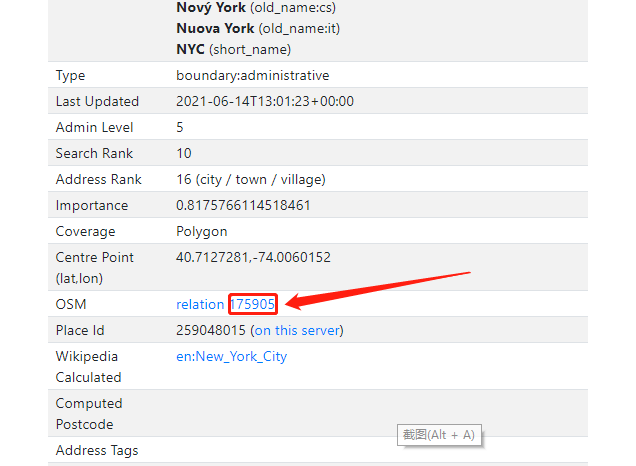
\includegraphics[width=0.4\textwidth]{./img/OSM ID.png} %插入图片,[]中设置图片大小,{}中是图片文件名
\caption{OSM 码} %最终文档中希望显示的图片标题
\label{Fig.OSM} %用于文内引用的标签
\end{figure}

在此网站输入OSM码\url{http://polygons.openstreetmap.fr/index.py},点击提交后就可以下载了。
\begin{figure}[H] %H为当前位置,!htb为忽略美学标准,htbp为浮动图形
\centering %图片居中
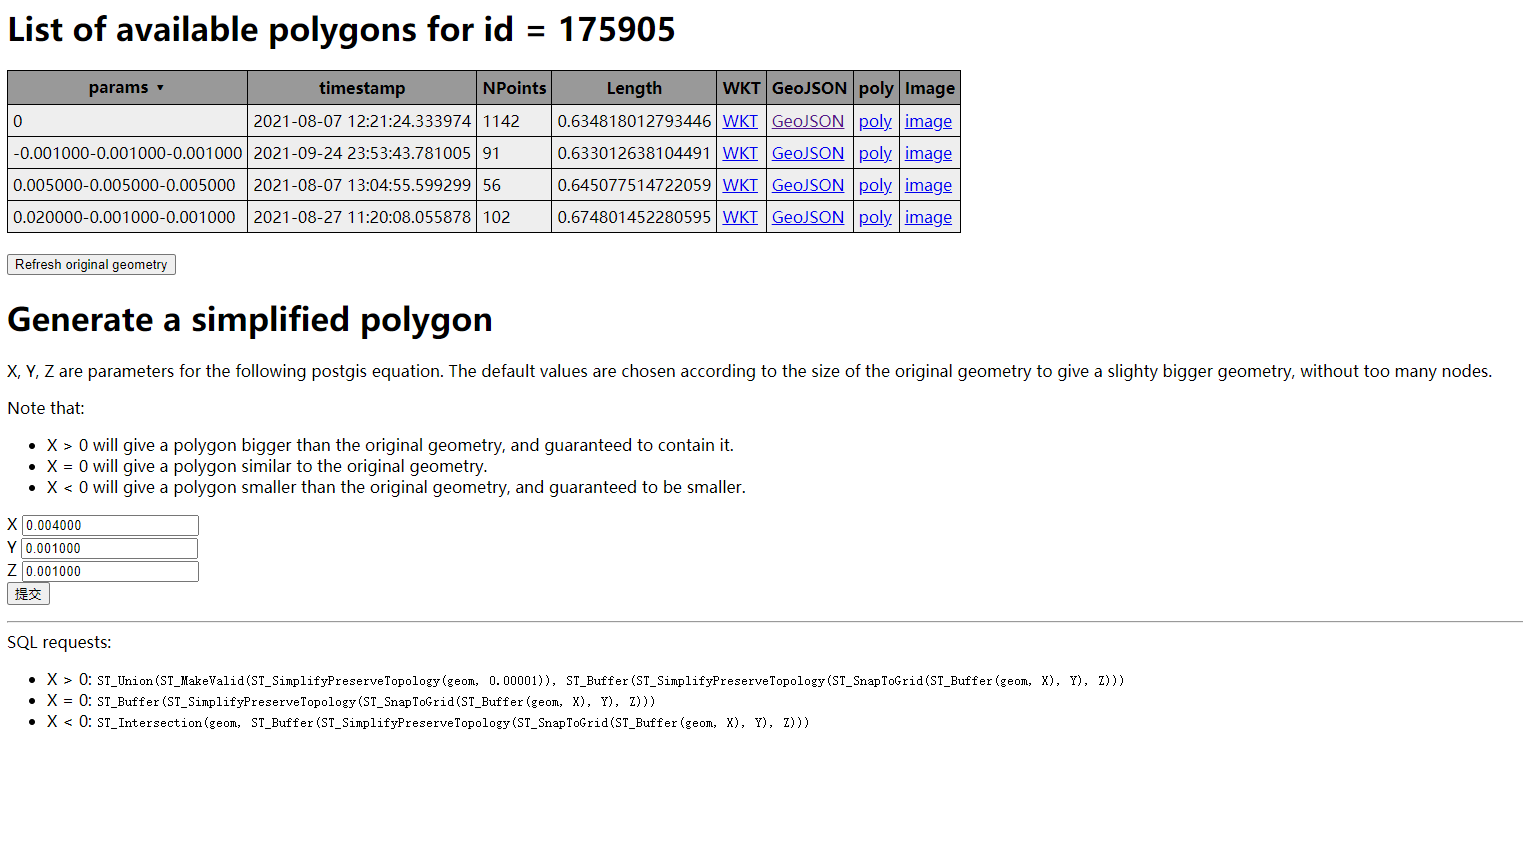
\includegraphics[width=0.4\textwidth]{./img/download.png} %插入图片,[]中设置图片大小,{}中是图片文件名
\caption{下载界面} %最终文档中希望显示的图片标题
\label{Fig.download} %用于文内引用的标签
\end{figure}

后续可以写一个方法,输入区域的名称后即可将该区域边界提取。

\subsubsection{判断方法}
由于New York城市是由多个点组成的一个不规则多边形,我们写了一个方法,用于判断某个经纬度坐标是否在New York这个城市里。此方法为射线法,步骤如下:
\begin{itemize}
\item[1)]从需要判断的点P向右引水平扫描线(即射线)。
\item[2)]计算此射线与多边形的交点个数c。
\item[3)]如果c为奇数,认为点P在多边形内;为偶数,则点P在多边形外。
\end{itemize}
如下图(a),c为奇数,所以P点在多边形外,图(b),c为偶数,所以P点在多边形内。


\begin{figure}[htbp]
\centering
\subfigure[P点在多边形外]{
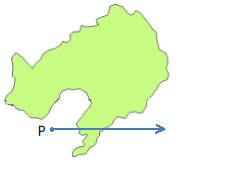
\includegraphics[width=0.3\textwidth]{./img/Ray_line_a.png}
%\caption{fig1}
}
\quad
\subfigure[P点在多边形内]{
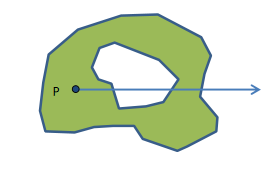
\includegraphics[width=0.3\textwidth]{./img/Ray_line_b.png}
}

\caption{射线法}
\end{figure}

在我们的数据集里,New York城市的边界是由很多个点(经纬度)组成的,我们可以把这些点连起来,就形成了一个多边形,再使用射线法去判断
。

我们的将此方法转化为程序的主要思路为:
\begin{itemize}
  \item [1)]
我们规定,点P为需要判断的点,$ x_p, y_p $分别为P的经度和纬度。$ N=\{P_n=(x_n,y_n)\mid n \in [0, k]\} $为New York城市的边界经纬度集合,其中k为New York城市经纬度的点的数量。

\item [2)]
按顺序将New York城市边界的每两个点连起来(如$ P_1, P_2 $或$ P_2, P_3 \cdots $),得到线段AB
\item [3)]
每次都用点P向右作射线,判断点P是否穿过线段AB
\item [4)]
如穿过,c加一,反之,c保持不变。
\item[5)]
直至后面将New York城市的所有点都判断后,再判断c的奇偶性,如c为奇数,则说明点P在多边形内,反之,点P在多边形外。
\end{itemize}
由于射线法本身存在缺陷,且在转化成代码时也会有相应的问题,我们在使用射线法前先进行了初步的判断以及排除一些情况:
\begin{itemize}
\item[1)]判断点P是否属于N,如是,则说明P在New York城市内。
\item[2)]判断点P是否属于线段AB上,如是,则说明P在New York城市内。(伪代码是否要给出来?)
\item[3)]点P正好位于线段AB的下端点,则在射线法里跳过此线段的判断。(怎么描述能更清楚?)
\item[4)]线段在射线的上方、线段在射线的下方、线段在射线的左方,则在射线法里跳过此线段的判断。


\end{itemize}
公式如下:

\[
isInRegion(N,P) = \begin{cases} in, & 2\nparallel \sum\limits_{n=1}^{k} M(P_n, P_{n+1},P)
 \\
out, & 2\parallel \sum\limits_{n=1}^{k} M(P_n, P_{n+1},P)
\end{cases}
\]
其中,k为New York城市经纬度的点的数量, $ M(P_n, P_{n+1},P) $的作用为计算每一条线段与P是否有交点,公式在此给出:
\[
M(P_n, P_{n+1},P) = \begin{cases}
0, & x_{meet}< x_p
 \\
1, & x_{meet}> x_p
\end{cases}
\]
\[
x_{meet} = x_n -\frac{x_n - x_{n+1}}{y_n - y_{n+1}}(y_n - y_p)
\]
其中,$ x_{meet} $为P点的射线与线段AB的交点的横坐标,其原理为三角形的相似性,原公式如下:
\[
\frac{x_n - x_{n+1}}{y_n - y_{n+1}}= \frac{x_n - x_{meet}}{y_n - y_p}
\]

\begin{figure}[H] %H为当前位置,!htb为忽略美学标准,htbp为浮动图形
\centering %图片居中
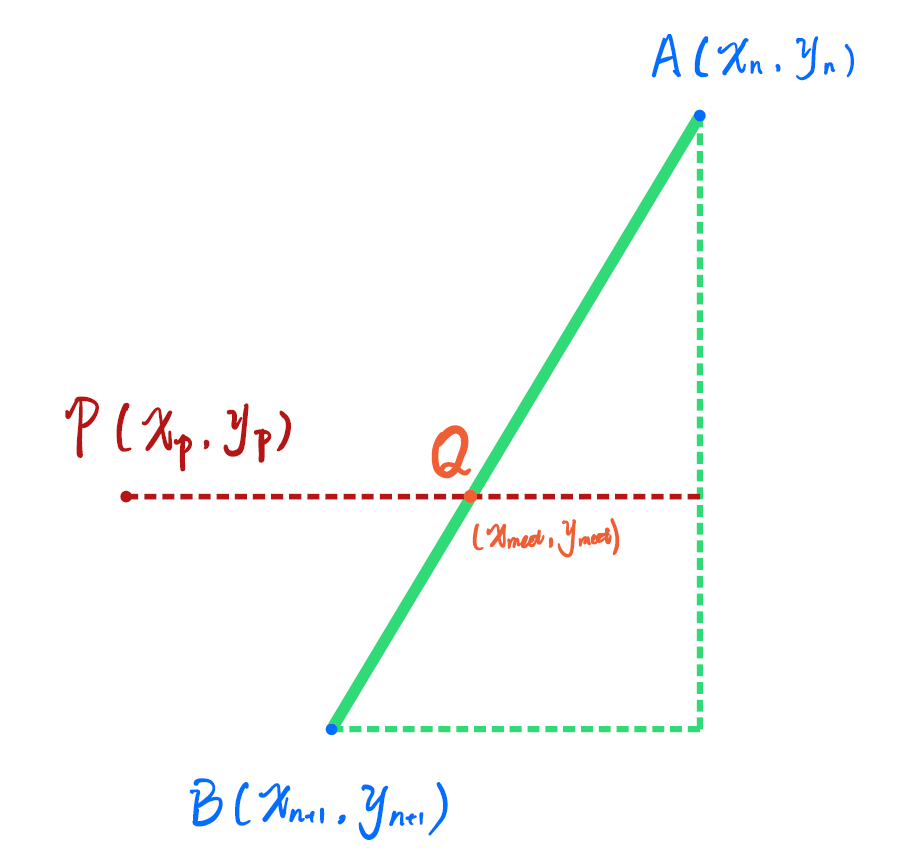
\includegraphics[width=0.4\textwidth]{./img/similar_triangles.png} %插入图片,[]中设置图片大小,{}中是图片文件名
\caption{similar triangles} %最终文档中希望显示的图片标题
\label{Fig.main2} %用于文内引用的标签
\end{figure}



在上面的公式里,$ isInRegion(N,P) $中,如果 $ \sum\limits_{n=1}^{k} M(P_n, P_{n+1},P) $能被2整除,说明c为偶数,所以我们通过射线法可以知道点P在该区域内,反之,则在该区域外。


%此外,由于射线法是有一定的缺陷的,当该点在多边形上时,并不能准确判定该点是否在多边形内,因此,我们在使用射线法前先进行简单判断,如果点P在多边形上,则认为该点是在该区域内,反之,则使用射线法进行进一步的判断。判断公式如下
%
%\IncMargin{1em}
%\begin{algorithm}[H]
%%\SetAlgorithmName{\color{red} \textbf{算法}}{}{}
%
%\SetKwData{Left}{left}\SetKwData{This}{this}
%\LinesNumbered
%\SetKwData{Up}{up}
%\SetKwFunction{Union}{Union}\SetKwFunction{FindCompress}{FindCompress}
%\SetKwInOut{Input}{Input}
%\SetKwInOut{Output}{output}
%\Input{Longitudes $ X $; \newline Latitudes $ Y $; \newline P \quad $ x_p, y_p $}
%\
%%\Output{A partition of the bitmap}
%%\BlankLine %间距
%%\emph{special treatment of the first line}\;
%\For{$ n=1,2,\ldots ,N $}{
%\uIf{$ x_p >= min(x_n, x_{n+1}) \quad  and \quad x_p <= max(x_n, x_{n+1})$}
%{\label{lt}
%\uIf{$ y_p >= min(y_n, y_{n+1}) \quad  and \quad y_p <= max(y_n, y_{n+1})$}
%{\label{lt}
%\uIf{$ (x_p - x_n)(y_{n+1}-y_n) - (x_{n+1}-x_n)(y_p - y_n) = 0 $}{\KwRet{$ True $}}
%}
%}}
%
%\caption{isInlinesegment Function}\label{isInlinesegment Function}
%\end{algorithm}\DecMargin{1em}
%
%
%公式解释,在判断一个点是否在一条线段上,有两个条件
%\begin{itemize}
%  \item [1)]
%  该点在以此线段为对角线的矩阵内(第一、第二个if判断条件)
%  \item [2)]
%  该点与此线段的其中一端相连形成的线段B,把此线段B与原线段求叉积,若叉积为0时(第三个if判断条件)
%\end{itemize}

    
